\documentclass{beamer} 
\usepackage{siunitx,booktabs,xcolor,xspace,multirow,graphicx,lipsum}
\usepackage[spanish,mexico,es-noindentfirst]{babel}
\usepackage[utf8]{inputenc}
\usepackage{tikz}
\usepackage{subcaption}
\usepackage[charter]{mathdesign}
\usetheme{Madrid}
\usepackage{tcolorbox}
\usepackage{hyperref}
\usepackage{rotating}
\usepackage{float}
\usepackage{venndiagram}
\usepackage{comment}
\usefonttheme{serif}

%\setbeamertemplate{frametitle}{
%  \begin{beamercolorbox}[wd=\paperwidth,ht=1cm, sep=0.25cm]{frametitle}
   % \begin{tikzpicture}[remember picture,overlay]
     % \node[anchor=north east] at (current page.north east) 
%{\includegraphics[height=0.75cm]
%{special_figures/logo_un_sinfondo.png}};
   % \end{tikzpicture}
   % \usebeamerfont{frametitle}\bfseries\insertframetitle
 % \end{beamercolorbox}}

\setbeamertemplate{caption}[numbered]
\setbeamercolor{frametitle}{bg=beamer_color,fg=white}
\setbeamercolor{author in head/foot}{bg=beamer_color,fg=white}
\setbeamercolor{title in head/foot}{bg=beamer_color,fg=white}
\setbeamercolor{date in head/foot}{bg=beamer_color,fg=white}
\setbeamercolor{titlelike}{parent=structure,bg=beamer_color,fg=white}
\setbeamertemplate{section in toc}[sections numbered]
\setbeamertemplate{subsection in toc}[subsections numbered]
\setbeamerfont{section in toc}{series=\bfseries}
\setbeamercolor{section in toc}{fg=black}
\setbeamercolor{caption name}{fg=blue}
\setbeamerfont{caption name}{series=\bfseries}
\setbeamerfont{caption}{size=\small}
%\setbeamercolor{bibliography entry author}{fg=black}
%\setbeamercolor{bibliography entry title}{fg=black} 
\setbeamertemplate{section in toc}{\inserttocsectionnumber.~\inserttocsection\par}
\setbeamertemplate{subsection in toc} {\hspace{1.5em}\inserttocsectionnumber.\inserttocsubsectionnumber~\inserttocsubsection\par}
\usepackage{ragged2e}
\usepackage{comment}

\title[\textbf{}]{\textbf{Informe estadístico Welcome Team}}
\author[\textbf{Informe de: WELCOME TEAM}] {\textbf{Para: Valentina Reyes \\ Melisa Ospina}}


\date{\textbf{26 de Dicembre, 2024}}
\renewcommand{\maketitle}{
\vspace{-0.5\baselineskip}

%\begin{center}
 %   \includegraphics[height=2.0cm]
%{special_figures/logo_uninorte.png}\hfill
    %\includegraphics[height=2.0cm]
%{special_figures/sello_institucional.jpg}\hfill
%\end{center}

%\vspace{20mm}

%\begin{center}
%    \textbf{}
%\end{center}

\vspace{-4mm}

\titlepage
\vspace{\baselineskip}
\begin{center}
    \small
    \vspace{-2.5\baselineskip}
    \textbf{Iglesia Boston Central}\\
    %Revisor 1: Nombre del primer revisor\\
    %Revisor 2: Nombre del segundo revisor\\
\end{center}
} 

% Definir color verde
% \definecolor{beamer_color}{RGB}{64, 145, 63}
% \definecolor{backframe_color}{RGB}{228, 242, 232}

% Definir color morado
\definecolor{beamer_color}{RGB}{112,49,148} 
\definecolor{backframe_color}{RGB}{235, 196, 245}
\begin{document}
%-----------------------%
%  DIAPOSITIVA  1       %
%-----------------------%
\begin{frame}
    \maketitle  
\end{frame}

%-----------------------%
%  DIAPOSITIVA  21      %
%-----------------------%
\subsection{}
\begin{frame}{Introducción}
\vspace{-0.9\baselineskip}
\begin{tcolorbox}[colback=backframe_color,colframe=beamer_color] 
Con la finalidad de hacer seguimiento al proceso desarrollado por el ministerio Welcome Team, se diseñó una encuesta para identificar factores a potencializar y fortalezas del proceso.
Para este informe, la encuesta se dirigió a las personas que sábado a sábado se reciben en nuestro ministerio y aquellas que nos fueron reportadas por otros ministerios de la iglesia que cooperan con Misión Josué.
\\\\
Este informe se basa en un análisis puramente descriptivo, el instrumento de medición fue un cuestionario que contó con 12 items y un espacio abierto para observaciones de los participantes.
\\\\
Se espera que a partir de sus resultados, se pueda tener una lectura más amplia del trabajo desarrollado y establecer metas futuras.

\end{tcolorbox}
\end{frame}




%-----------------------%
%  DIAPOSITIVA  22      %
%-----------------------%

\subsection{}
\begin{frame}{Objetivos}
\vspace{-0.9\baselineskip}
\begin{tcolorbox}[colback=backframe_color,colframe=beamer_color,title= ] 
\begin{itemize}
    \item Describir los participantes que de forma regular se reciben en Welcome Team y asisten a Misión Josué.
    \item Realizar seguimiento a los procesos desarrollados al interior de Welcome Team.
    \item Evaluar e identificar aspectos de mejora en los procesos dirigidos por el ministerio.
\end{itemize}


\end{tcolorbox}
\end{frame}


%-----------------------%
%  DIAPOSITIVA  23      %
%-----------------------%

\subsection{}
\begin{frame}{Metodología}
\vspace{-0.9\baselineskip}
\begin{tcolorbox}[colback=backframe_color,colframe=beamer_color,title= Elección de la muestra] 
La muestra seleccionada es no probabilistica debido a que inicialmente es un estudio exploratorio del ministerio y en segundo lugar, las respuestas al cuestionario estaban en función de las personas que accedieron a responder. A razón de lo anterior, las afirmaciones e interpretaciones realizadas en este documento no van más allá de los participantes que respondieron. 
\\\\
Como criterio de selección los participantes debian ser jóvenes con edades entre los 14 y 28 años y cuyos datos se encontraran completos, así las cosas; se analizó la base de datos  y se depuró a una lista de 100 personas que conformaron la población; eliminando personas repetidas o aquellas cuyos números de teléfono estaban incompletos. La muestra final fue de 19 personas que respondieron el cuestionario. 
\end{tcolorbox}
\end{frame}



%-----------------------%
%  DIAPOSITIVA  24      %
%-----------------------%
\subsection{}
\begin{frame}{}
\vspace{-0.9\baselineskip}
\begin{tcolorbox}[colback=backframe_color,colframe=beamer_color,title= Instrumentos: cuestionario] 
Con la finalidad de responder a los objetivos planteados, se optó por elaborar un cuestionario vía Google Forms el cual fue enviado mediante WhatsApp; siendo muy útil en términos de la distancia con los participantes. Este cuestionario constaba de 12 items y de un espacio abierto para comentarios. Este cuestioario resultó ser optimo debido a su facil elaboración, bajo coste y rapidez para responder por parte de los participantes.
\end{tcolorbox}
\end{frame}



%-----------------------%
%  DIAPOSITIVA  25      %
%-----------------------%
\subsection{}
\begin{frame}{}
\vspace{-0.9\baselineskip}
\begin{tcolorbox}[colback=backframe_color,colframe=beamer_color,title= Técnicas: Análisis Univariado y Bivariado] 
Una vez recolectada la información se procedió a realizar los respectivos análisis estadísticos. Para esto se utilizaron las medidas de tendencia central y dispersión acompañadas de las respectivas visualizaciones y pruebas de hipótesis en el caso de ser necesarias.  
    
\end{tcolorbox}
\end{frame}



%-----------------------%
%  DIAPOSITIVA  26      %
%-----------------------%
\subsection{}
\begin{frame}{RESULTADOS}
\vspace{-0.9\baselineskip}
\begin{tcolorbox}[colback=backframe_color,colframe=beamer_color,title= ] 
Analizando la edad de los participantes se encontró que la edad mínima fue de 14 años y la edad máxima fue de 23 años. El promedio de edad fue de 18.21 años con una desviación de $\pm 2.68$ años. Por sexo,  se puede observar que la mediana de la edad para las mujeres es de 18 años y por parte de los hombres al rededor de los 19.5 años.


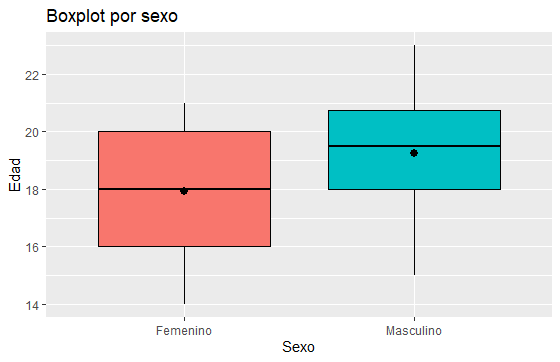
\includegraphics[width=0.65\linewidth]{special_figures/Rplot.png}
    
\end{tcolorbox}
\end{frame}


%-----------------------%
%  DIAPOSITIVA  27      %
%-----------------------%
\subsection{}
\begin{frame}{}
\vspace{-0.9\baselineskip}
\begin{tcolorbox}[colback=backframe_color,colframe=beamer_color,title= ] 
En relación a la participación de los encuestados, se encontró que 15 fueron mujeres y 4 fueron hombres lo que corresponde al 79\% y 21\% respectivamente para cada categoría.  

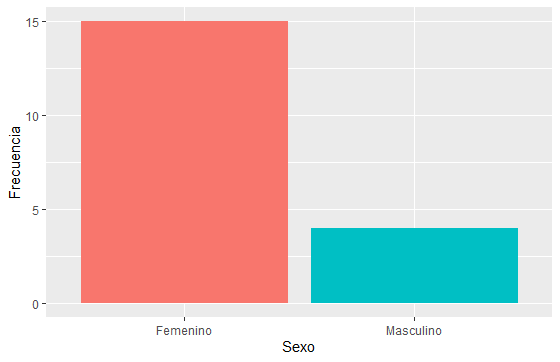
\includegraphics[width=0.9\linewidth]{special_figures/Rplot02.png}
    
\end{tcolorbox}
\end{frame}



%-----------------------%
%  DIAPOSITIVA  28      %
%-----------------------%
\subsection{}
\begin{frame}{}
\vspace{-0.9\baselineskip}
\begin{tcolorbox}[colback=backframe_color,colframe=beamer_color,title=] 
En relación a la asitencia los días sábados a Misión Josué se encontró que el 79\% de los participantes indicaron que sí (15 personas) y solo el 21\% respondió que no (4 personas). Además, se puede apreciar que para ambos casos la proporción de mujeres es mucho mayor. 
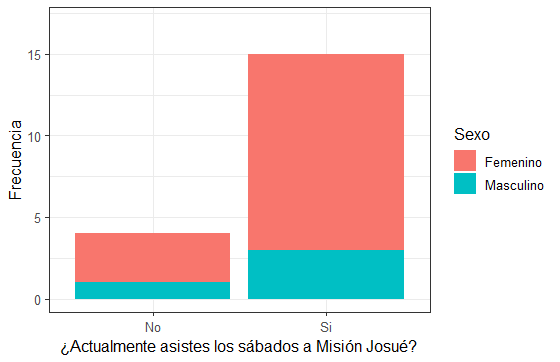
\includegraphics[width=0.8\linewidth]{special_figures/Rplot03.png}
    
\end{tcolorbox}
\end{frame}






%-----------------------%
%  DIAPOSITIVA  30      %
%-----------------------%

\subsection{}
\begin{frame}{}
\vspace{-0.9\baselineskip}
\begin{tcolorbox}[colback=backframe_color,colframe=beamer_color,title=] 

En relación con la frecuencia de asistencia los días sábados se observa que el 21.05 \% no está asistiendo actualmente, el 52.6 \% asiste de manera frecuente y solo el 26.35 \% asiste de forma esporádica. 
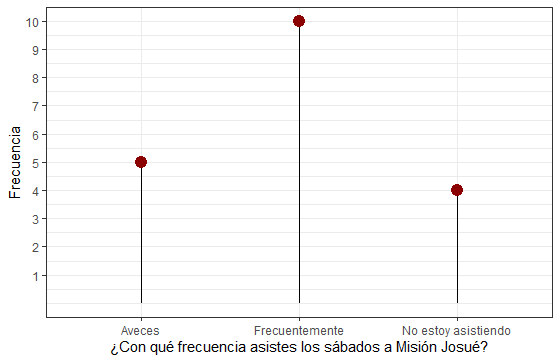
\includegraphics[width=0.9\linewidth]{special_figures/Rplot01_1.png}
\end{tcolorbox}
\end{frame}


%-----------------------%
%  DIAPOSITIVA  31      %
%-----------------------%

\subsection{}
\begin{frame}{}
\vspace{-0.9\baselineskip}
\begin{tcolorbox}[colback=backframe_color,colframe=beamer_color,title=] 

Por otro lado, al preguntar sobre su vinculación a un grupo de conexión (CNX) el 52.6 \% respondió que si y el 47.4 \% respondió que no. 
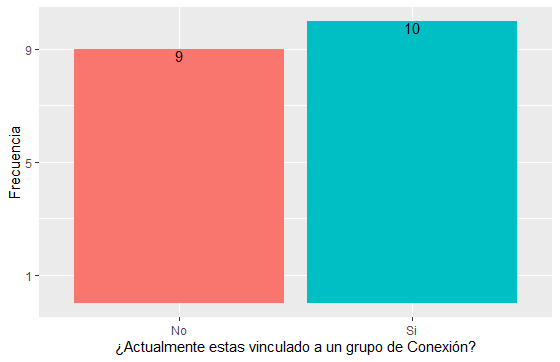
\includegraphics[width=0.8\linewidth]{special_figures/Rplot05.png}
\end{tcolorbox}
\end{frame}






%-----------------------%
%  DIAPOSITIVA  32      %
%-----------------------%
\subsection{}
\begin{frame}{}
\vspace{-0.9\baselineskip}
\begin{tcolorbox}[colback=backframe_color,colframe=beamer_color,title=] 

Haciendo seguimiento a la vinculación de los asistentes a un grupo de CNX  el 63.1 \% respondió de manera afirmativa y solo el 36.9 \% respondió que no.
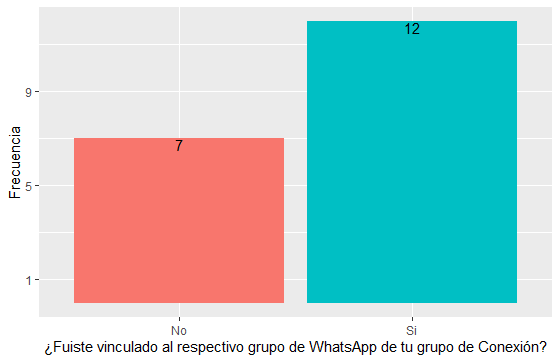
\includegraphics[width=0.8\linewidth]{special_figures/Rplot06.png}
\end{tcolorbox}
\end{frame}


%-----------------------%
%  DIAPOSITIVA  33      %
%-----------------------%
\subsection{}
\begin{frame}{}
\vspace{-0.9\baselineskip}
\begin{tcolorbox}[colback=backframe_color,colframe=beamer_color,title=] 

En relación a la asistencia actual a los grupos de CNX se cuenta con un porcentaje de asistencia bastante bajo, solo el 31.5 \% respondió que asiste de manera frecuente y el 21.05 \% asiste de manera esporádica, contra un 47.45 \% que manifestó no estar asistiendo. 
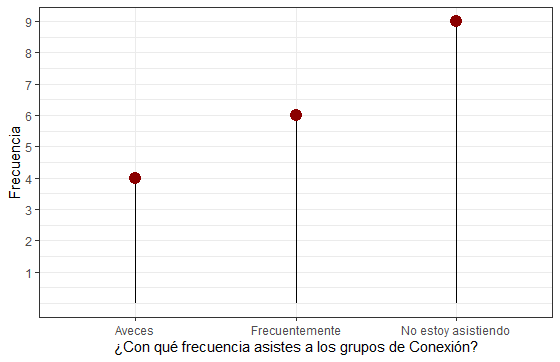
\includegraphics[width=0.7\linewidth]{special_figures/Rplot01_2.png}
\end{tcolorbox}


\end{frame}

%-----------------------%
%  DIAPOSITIVA  34      %
%-----------------------%
\subsection{}
\begin{frame}{}
\vspace{-0.9\baselineskip}
\begin{tcolorbox}[colback=backframe_color,colframe=beamer_color,title=] 
En relación al seguimiento por consejeria el 68.4 \% respondió de manera negativa y solo un 31.6 \% respondiio de forma afirmativa a esta pregunta. 

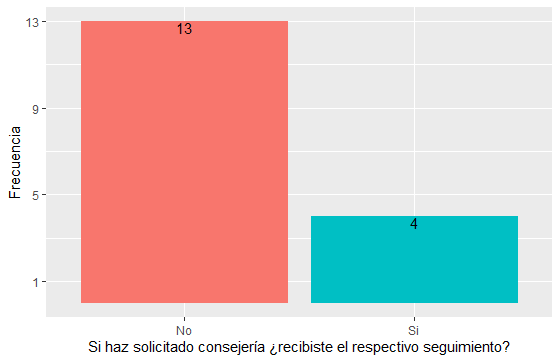
\includegraphics[width=0.8\linewidth]{special_figures/Rplot08.png}
\end{tcolorbox}
\end{frame}

%-----------------------%
%  DIAPOSITIVA  35      %
%-----------------------%
\subsection{}
\begin{frame}{}
\vspace{-0.9\baselineskip}
\begin{tcolorbox}[colback=backframe_color,colframe=beamer_color,title=] 
En relación a su participación en el retiro el Dios de mi Historia, solo el 15.7 \% asistió contra un 84.3 \% que no participó del mismo. Esto probablemente se deba a que la mayoría que respondió la encuesta fueron individuos que se integraron muy posterior al retiro.
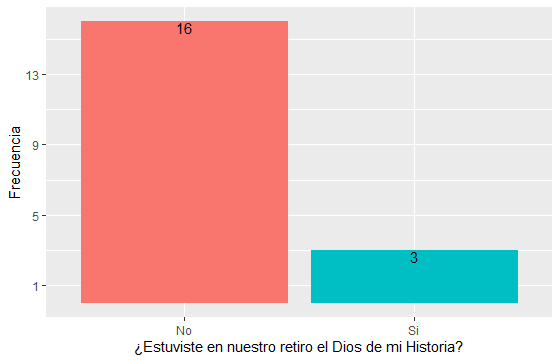
\includegraphics[width=0.8\linewidth]{special_figures/Rplot09.png}
\end{tcolorbox}
\end{frame}


%-----------------------%
%  DIAPOSITIVA  46     %
%-----------------------%
\subsection{}
\begin{frame}{}
\vspace{-0.9\baselineskip}
\begin{tcolorbox}[colback=backframe_color,colframe=beamer_color,title=] 
En relación a los medios mas utilizados para estar al pendientes de las actividades de Misión Josué la gran mayoría con un 36.8 \% respondió que Instagram, mediante grupos de CNX solo un 26.3 \%, porcentaje compartido con los anuncios el el servicio de jóvenes y solo un 10.6\% respondió de manera voz a voz. 
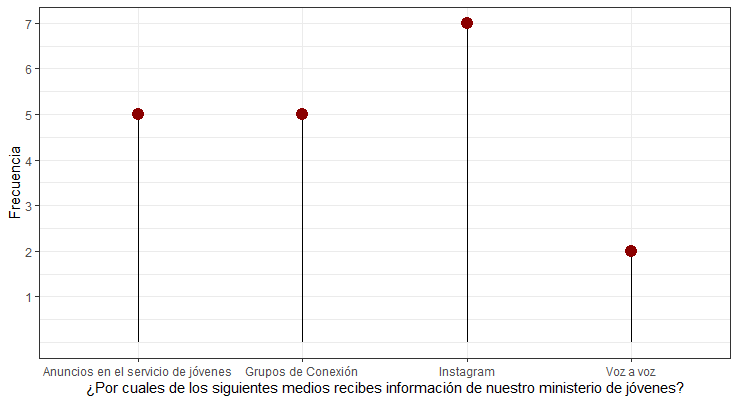
\includegraphics[width=0.95\linewidth]{special_figures/Rplot01_3.png}
\end{tcolorbox}
\end{frame}



%-----------------------%
%  DIAPOSITIVA  47     %
%-----------------------%
\subsection{}
\begin{frame}{}
\vspace{-0.9\baselineskip}
\begin{tcolorbox}[colback=backframe_color,colframe=beamer_color,title= Comentarios de los participantes] 
\begin{itemize}
    \item Más integración con los grupos 
    \item Donde podría conectarme a los servicios ya que no puedo asistir presencial por que me cambie de ciudad 
    \item Me encanta ir los sábados y ser parte de misión Josué , les doy muchas gracias por ser tan amables conmigo
    \item Sigan trabajando así, Dios salvó mi vida atravez de su gran desempeño en los trabajos del Reino.

\end{itemize}
\end{tcolorbox}
\end{frame}





%-----------------------%
%  DIAPOSITIVA  48     %
%-----------------------%
\subsection{}
\begin{frame}{}
\vspace{-0.9\baselineskip}
\begin{tcolorbox}[colback=backframe_color,colframe=beamer_color,title= Comentarios de los participantes] 
\begin{itemize}
   \item Siempre hago lo posible por ir pero  al aveces que mi mamá  se pone muy mal o mi hermano que tiene problema de esquizofrenia  y me toca quedarme   pero   me encantaría ir   para reparar mi  corazón. 

    \item creo que sería chevre que los sábados fueran más dinámico,  que hubieran espacios para conocerse con gente de otros grupos de conexión, también actividades solo para mujeres y solo para hombres y más espacios de dialogo después de la enseñanza. 
\end{itemize}
\end{tcolorbox}
\end{frame}




%-----------------------%
%  DIAPOSITIVA  49     %
%-----------------------%
\subsection{}
\begin{frame}{}
\vspace{-0.9\baselineskip}
\begin{tcolorbox}[colback=backframe_color,colframe=beamer_color,title= Pruebas de hipótesis] 
Con la finalidad de profundizar el análisis en función de los datos obtenidos, se encontró que:

\begin{enumerate}
    \item Aplicando la prueba Shapiro-Wilk debido al tamaño pequeño de la muestra $(n=19)$, en relación a la edad esta sigue una distribución normal con $valor p = 0.098$ y significancia de $\alpha = 0.05$. Lo que significa que la mayoría de las personas en la muestra tienen edades cercanas al promedio. 
    \item Dado que las frecuencias esperadas fueron menor a 5, se optó por la prueba de independencia de Fisher,encontrando que existe una relación significativa entre asistir los sábados a Misión Josué y estar vinculado a un grupo de conexión con $valorp= 0.03251$ y significancia de $\alpha = 0.05$
\end{enumerate}
\end{tcolorbox}
\end{frame}




%-----------------------%
%  DIAPOSITIVA  50     %
%-----------------------%
\subsection{}
\begin{frame}{}
\vspace{-0.9\baselineskip}
\begin{tcolorbox}[colback=backframe_color,colframe=beamer_color,title= Pruebas de hipótesis] 


\begin{enumerate}
    \item Mediante la prueba de independencia de Fisher, no se encontró evidencia significativa entre las personas que aisten los sábados a Misión Josué y manifestaron que no habian recibido consejeria $valorp= 0.5193.$ y significancia de $\alpha = 0.05$
    \item De forma análoga se encontró que no hay evidencia significativa para afirmar que existe relación entre el género y las personas de la muestra que asisten a Misión Josué, $valor p=1.0$ y significancia de $\alpha = 0.05$
\end{enumerate}
\end{tcolorbox}
\end{frame}

%-----------------------%
%  DIAPOSITIVA  51     %
%-----------------------%
\subsection{}
\begin{frame}{}
\vspace{-0.9\baselineskip}
\begin{tcolorbox}[colback=backframe_color,colframe=beamer_color,title= Conclusiones] 
A partir de los resultados obtenidos se permiten establecer las siguientes conclusiones:

\begin{enumerate}
    \item El género femenino ocupa una mayor proporción en la muestra, aspecto que se puede corroborar al interior del ministerio incluso si la muestra fuera mayor. 
    \item A nivel de la muestra la mayoría continua asistiendo a Misión Josué, sin embargo, no se debe confundir la proporción de personas que asisten a Misión Josué y la proporción de personas que asisten a Misión Josué y han presentado un seguimiento por Welcome Team, donde esto último es el interes especial. En este orden de ideas, es necesario el seguimiento cuantitativo para poder hacer comparaciones y medir el crecimiento real. Actualmente de las 100 personas que conformaron la población que ha pasado por Welcome Team, solo 19 respondieron, es decir, solo el 19\%. Y solamente el 15 \% respondió que actualmente continua asistiendo. Donde esta sería la proporción para el año 2024. 
\end{enumerate}
\end{tcolorbox}
\end{frame}



%-----------------------%
%  DIAPOSITIVA  52     %
%-----------------------%
\subsection{}
\begin{frame}{}
\vspace{-0.9\baselineskip}
\begin{tcolorbox}[colback=backframe_color,colframe=beamer_color,title= Conclusiones] 

\begin{enumerate}
    \item Se pudo apreciar que solo un poco mas de la mitad de la muestra (52.6 \%) está vinculada a un grupo de CNX. Donde solo el 21.05 \% manifestó que asiste de manera frecuente. Seria recomendable que los líderes de los grupos de CNX puedan hacer un seguimiento de las personas anexadas a sus grupos, ¿por qué han faltado? ¿qué necesitan? etc.
    \item Según la muestra la consejería es uno de los aspectos que no tiene los mejores indicadores, con un 68.4\%  han manifestado no recibirla en caso de solicitarla. 
    \item En relación a la asistencia a Misión Josué y la asistencia al retiro el Dios de mi Historia, solo se encontraron tres personas. Sin embargo, este aspecto no puede considerarse negativo como tal debido a que las personas que respondieron la encuesta se integraron a partir del mes de septiembre a la iglesia.  
\end{enumerate}
\end{tcolorbox}
\end{frame}





%-----------------------%
%  DIAPOSITIVA  53    %
%-----------------------%
\subsection{}
\begin{frame}{}
\vspace{-0.9\baselineskip}
\begin{tcolorbox}[colback=backframe_color,colframe=beamer_color,title= Conclusiones] 

\begin{enumerate}
    \item En relación a las formas de hacer seguimiento a las actividades del ministerio, estas son variadas y es el Instagram el que mantiene mayor visibilidad. 
    \item A partir de los comentarios de los participantes estos no mantinen una misma línea y van desde sugerencias hasta agradecimeintos. Lo cierto esque constituyen un aspecto fundamental lo que las personas perciben acerca del ministerio, sus condiciones de vida y la permanencia en el mismo. 
    \item En relación a la edad, estas presentaron una variación desde los 14 a los 23 años, no hubieron datos atípicos por encima o debajo de estos valores. Por lo que a partir de la normalidad en la muestra, el ministerio tiende a orientarse entre edades cercanas a los 18 y 20 años de edad lo que refleja es su rango etario de mayor prioridad. 
\end{enumerate}
\end{tcolorbox}
\end{frame}


%-----------------------%
%  DIAPOSITIVA  54     %
%-----------------------%

\subsection{}
\begin{frame}{}
\vspace{-0.9\baselineskip}
\begin{tcolorbox}[colback=backframe_color,colframe=beamer_color,title= Conclusiones] 

\begin{enumerate}
    \item Un aspecto importante a partir de las pruebas de hipótesis es la relación entre asistir a Misión Josué y estar en un grupo de CNX.  Este aspecto es clave y debe seguir fortaleciendose en el ministerio; pues permite la integración de jóvenes, genera lazos de amistad y creciemiento. 
    \item Si bien no se encontró asociación entre el género de las personas y su asistencia al ministerio, quizá con una muestra mayor este resultado pueda invertirse.   
\end{enumerate}
\end{tcolorbox}
\end{frame}




%-----------------------%
%  DIAPOSITIVA  55      %
%-----------------------%

\subsection{Cuadros de texto}
\begin{frame}{}
\vspace{-0.9\baselineskip}
\begin{tcolorbox}[colback=backframe_color,colframe=beamer_color,title= Limitaciones] 

Como limitaciones de este estudio se hace énfasis en el tamaño de la muestra que fue menor al esperado. Cabe resaltar que las afirmaciones aquí planteadas tienen por límite la muestra misma y cualquier otra afirmación seria una hipótesis pendiente por validar con la evidencia empirica.

Este estudio es inicial y exploratorio; por ende susceptible a mejoras y recomendaciones tanto en el diseño de los instrumentos hasta el análisis técnico. Se espera que pueda servir de insumo para el crecimiento del ministerio y la ordenación de objetivos y metas. Los resultados aquí mostrados reflejan el trabajo y compromiso de cada uno de sus miembros y líderes. 
\\\\
Este trabajo no fuera sido posible sin la colaboración de Keyla Gonzalez, Silvana Suarez, Samir Arévalo, Alejandro Cortez, Melu Ospina, Abraham, Estefani Uribe y Valentina Reyes. 
\end{tcolorbox}
\end{frame}



%-----------------------%
%  DIAPOSITIVA  9     %
%-----------------------%

\section{Referencias}
%\begin{frame}[allowframebreaks]{Bibliografía} 
%\bibliographystyle{acm}
%\bibliography{biblio}
%\end{frame}
\begin{frame}
    \maketitle
\end{frame}
\end{document}